\section{Contribution}
\label{sec:contribution}

In the scope of this thesis, $REPLACE_WE$ developed FESDData and FESDModel, or Fault estimation for Skeleton detection for data collection and model creation. FESDData is the tool that allows $REPLACE_US$ to record, analyse and populate it with pose data using Nuitrack. 

FESDData is a tool that is designed to be easy to use and that can be used by anyone, and without much need for setup or tweaking. It allows for the rapid capture of RGBD datasets with pre-labeling of multiple different recordings. The parameters can be adapted to capture datasets for many different application, e.g. Action detection.

FESDModel is the model which $REPLACE_WE$ developed in the scope of this thesis. It utilises the data recorded using FESDData.

The code of this thesis is available on GitHub\footnote{\url{https://github.com/LeonardoPohl/FESD}}. The repository is divided into two major parts, FESDData, which contains the C++ implementation of the dataset recorded, FESDModel, which contains the implementation of the model, as well as the Jupyter notebook that was used to train the model. Additionally there is this thesis and all related figures.

\subsection{Developed Software}

\textit{\textbf{UNSURE} Should I write about the software, explain the OpenGL implementation, the ImGui GUI and so on?}
\textit{\textbf{TODO} Change Screenshots to light mode to be consistent with the rest of the thesis (can wait until screenshots are final)}

\begin{figure}[ht]
  \centering
  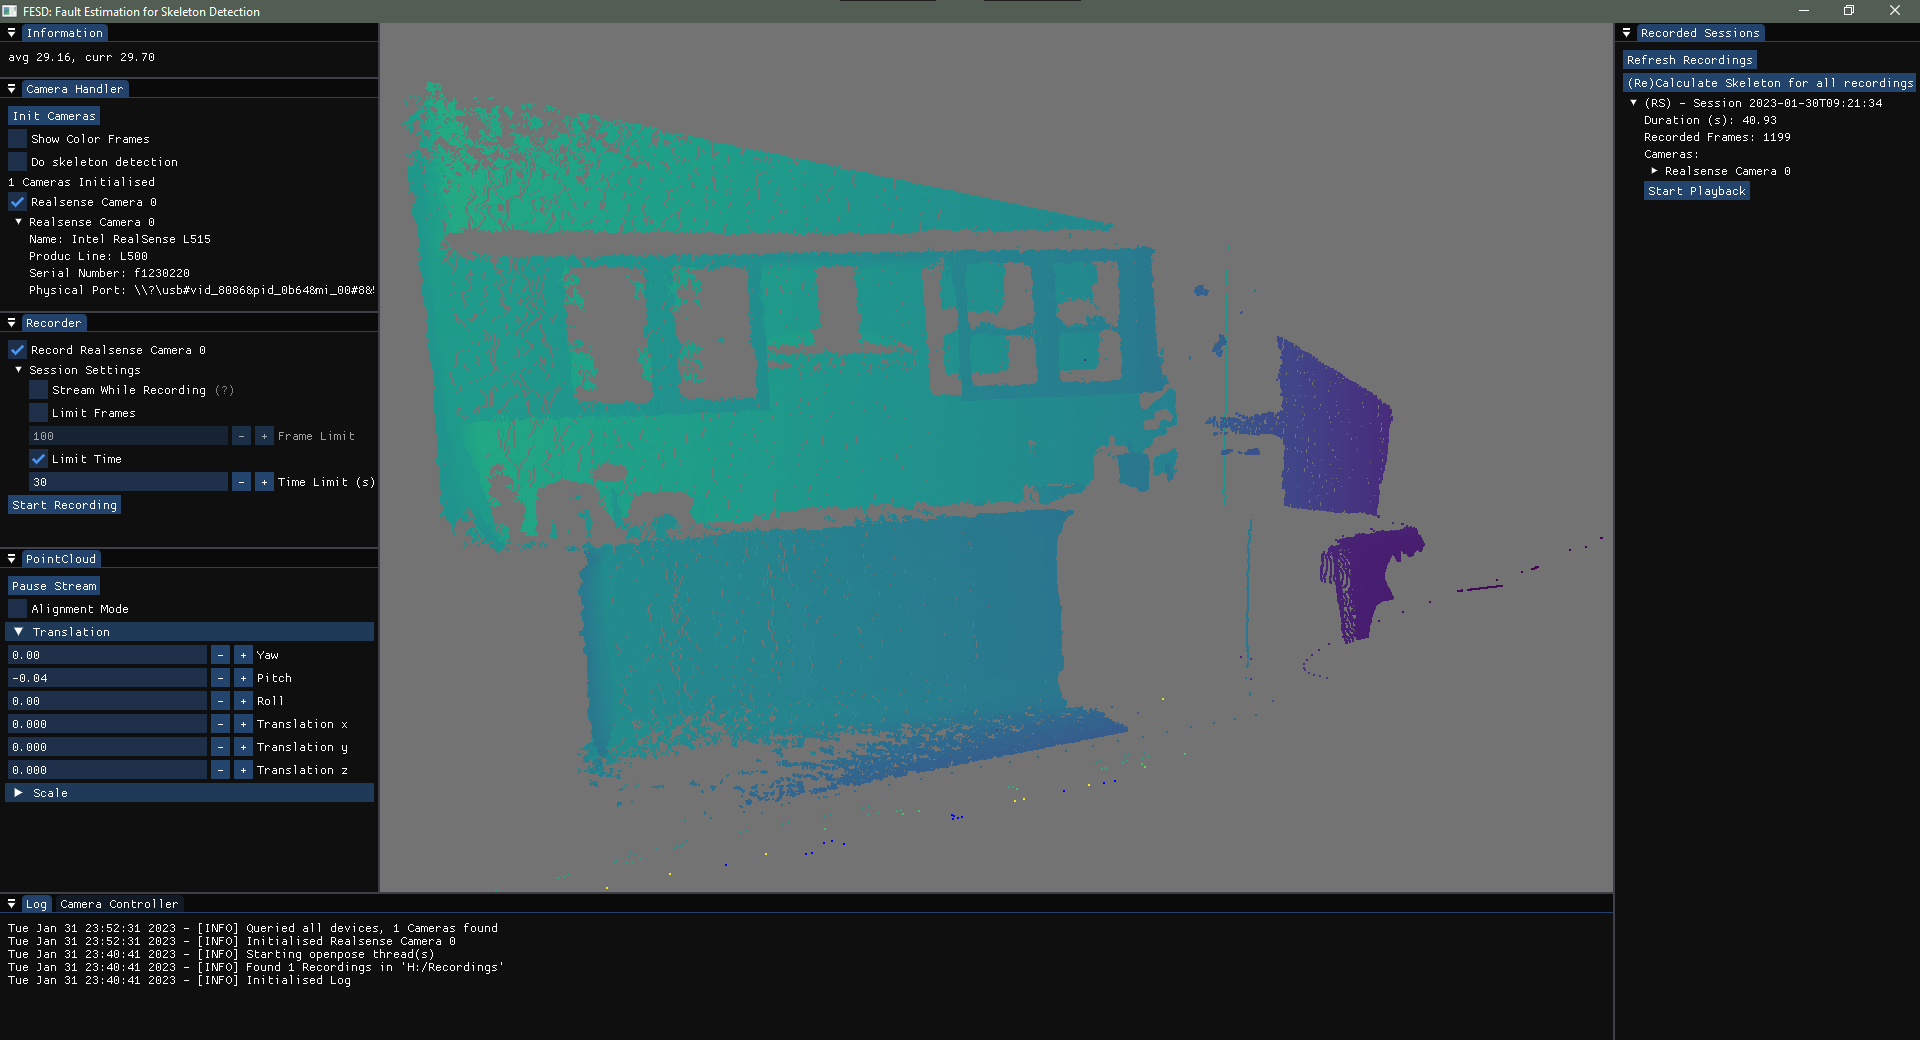
\includegraphics[width=\linewidth]{figures/FESD/all.png}
  \caption[FESDData GUI]{A screenshot of the FESDData GUI streaming a point cloud. The GUI is used to record, playback, visualise and label the data streams from RGBD cameras. The FESDData Gui is written in C++ using the ImGui framework. The point cloud is visualised using OpenGL and a glsl shaders.}
  \label{fig:stream_gui}
\end{figure}

\subsection{Possible applications}

FESD might find several different areas of application in the future. Firstly, the trained model can be used to assist in developing games and other applications that utilise Human Pose estimation. In its simplest application it may be used to warn users of possible errors when the skeleton is not detected correctly. In more advanced cases the information provided by the model could be used to attempt to fix joints through joint position interpolation and prediction rather than using the faulty joint. Moreover, multiple human pose estimators could be considered resulting in an overall more robust human pose estimation.

Furthermore, if the model proves to have a high accuracy for a specific use-case, it could be used to train a better pose detector in the same way as it is proposed by Jo\~ao Carreira et al. in \cite{IterativeErrorFeedback}.

The dataset and the dataset recorder may also be used to further the model development for fault estimation and it can also find application in other areas. The dataset in and of itself can be used for action detection. The exercises are predefined and can be recorded and automatically labeled by FESDData, thereby making it fairly simple to record large amounts of data without requiring a large amount of human work.